\documentclass{ituthesis}
\usepackage{hyperref}
\usepackage[]{float} 

\settitle{The Practical Guide to Levitation}
\setauthor{Ahmad Salim Al-Sibahi}
\setsupervisor{Dr. Peter Sestoft}
\setextrasupervisor{David R. Christiansen}
\setdate{September 1, 2014}

\begin{document}
%\selectlanguage{danish}

\frontmatter

\thetitlepage
\newpage

\chapter*{Abstract}
Goal: Implementation of levitation in a realistic setting, with practical performance benefits.

\cleardoublepage
\setcounter{tocdepth}{1}
\tableofcontents

\mainmatter

%from memoir documentation:
%TeX tries very hard to keep text lines justified while keeping the interword spacing as constant as possible, but sometimes fails and complains about an overfull hbox.
%The default mode for LaTeX typesetting is \fussy where the (variation of) interword spacing in justified text is kept to a minimum. Following the \sloppy declaration there may be a much looser setting of justified text.
%Additionally the class provides the \midsloppy declaration which allows a setting somewhere between \fussy and \sloppy.
%fewer overfull lines than \fussy, and fewer obvious large interword spacing than with \sloppy.
%the memoir manual also uses \midsloppy!
\midsloppy
% try harder to avoid widows and orphans
\sloppybottom

\chapter{Introduction}
\label{cha:Intoduction}
\section{Context}
\label{sec:Context}
Tradtionally, a core part of functional programming is the idea of algebraic datatypes such as booleans, natural numbers, lists, trees, and other types of inductive structures. These datatypes are often simple to work with since the possible cases are known, and the inherent design towards purity ensures that
most functions stay declarative which makes programs easier to reason about.

While it is often the case that functions must be tailored specifically to a certain datatype, in certain cases it often seems as we are repeating ourselves such as in the cases of boolean structural equality or textual conversions.
In fact it almost seems like we could instruct a computer to write the function for us, or rather it seems that it is possible to write a function over the structure of the datatype definition which the computer could use to derive
actual function for particular datatypes.

Enter the world of \textit{generic programming}, or colloquially \textit{functional metaprogramming}, where the target data is the datatype describing the structure of other datatypes which is often called the \textit{description}.
While generic programming indeed sounds promising, there has usually been issues regarding usability and performance in traditional functional languages such as Haskell. 
First of all, generic programming often requires special language extensions to encode the datatype description which further complicates things; otherwise, the description might be constructed incorrectly and require the programmer to handle weird edge cases.
Secondly, there is often some kind of discrepancy between ordinary programming and generic programming with generic programming almost requiring an orthogonal type-level style of programming; thus making it hard for the ordinary programmer to exploit.
Finally, due to the way generic programs are applied abstractly to datatypes instead of fitted specifically, there is often a large amount of overhead which sometimes cannot be optimised away since it is hard to safely perform arbitrary function transform; hence, generic programming usually is not considered an option for performance critical applications.

In dependently-typed languages such as Idris or Agda however, it seems that many of the issues can be mitigated.
Particularly, due to the nature of dependently-typed languages and the Curry-Howard isomorphism, it is possible to encode proofs in datatypes, and as such design the datatype description such that all values of that type are correct by construction.
More interestingly, such as the one shown by Dagand et al. in `The Gentle Art of Levitation' it is possible to build a complete typesystem which is able to convert values of the descriptions to ordinary types and is even powerful enough to describe the datatype description itself.
As such, in the Levitation-system generic programming can be achieved fully using ordinary programming techniques.

\subsection{Anatomy of a Datatype}
\label{sub:AnatomyofaDatatype}
A question the reader might have now is then how does a datatype description look, since that might not be completely obvious. To better understand however, let us start by investigating what a typical datatype is composed by.

\begin{figure}[ht]
\begin{center}
    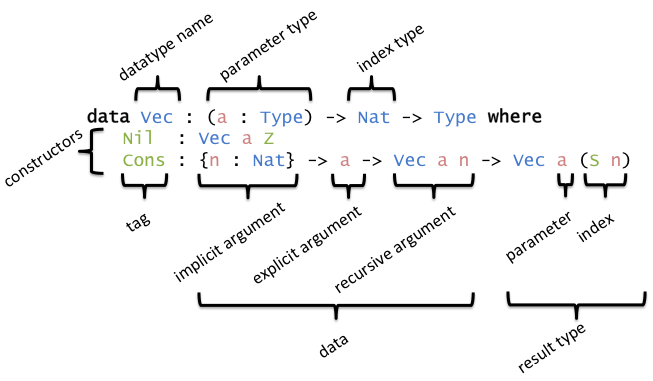
\includegraphics[scale=0.5]{Figures/AnatomyOfADatatype.png}
\end{center}
\caption{Annotated Components of a Datatype Declaration}
\label{fig:anatomydatatype}
\end{figure}

In Figure~\ref{fig:anatomydatatype}, I present an annotated version of a typical dependently-typed datatype that represents length-indexed lists, or vectors. While many things might initially seem trivial, it is nonetheless important to get a precise definition
on how a datatype is defined; especially, when that is the target structure for our future algorithms.

To describe the type constructor of a datatype, three components are needed: the name of the datatype, types of any possible parameters, and finally, since this is a dependently-typed language, the types of indicies of the datatype. In the figure it is notable that it seems there is no difference between a parameter type or an index type, but that is because
Idris figures this out automatically (unlike other dependently-typed languages).\footnote{If the argument to a type constructor doesn't change in the data constructor declarations Idris considers that a parameter, and otherwise an index.}

In addition to the type constructor, most datatypes contain one or more data constructors which provides a way to store the actual data. Similarly to a type constructor, a data constructor also needs a name, also called the \textit{tag} of the constructor.
Following the tag, the data constructor declaration contains the types of the arguments stored in the constructor and resulting type which must be the same as the datatype we are currently declaring.
In our example two constructors are declared, \texttt{Nil} and \texttt{Cons}.
Since \texttt{Nil} doesn't hold any data, the declaration only shows the resulting type which is \texttt{Vect a Z} (i.e. it constructs a list of length zero).
\texttt{Cons} is more interesting since it contains three different types of arguments: an implicit arguments of a different type, an explicit arguments of a different type, and an explicit argument to the type itself (recursive argument), with the resulting type being \texttt{Vect a (S n)} (i.e. it constructs a list of length one greater than the input recursive argument).
As the reader might have noticed the index of the resulting type of \texttt{Nil} is different from the index of the resulting type of \texttt{Cons}, while the parameters are seamingly the same.

\subsection{A Description for Datatypes}
\label{sub:ADescriptionforDatatypes}
After understanding how datatypes are structured, it is now possible to try and construct a suitable description datatype. Figure~\ref{fig:descriptiondatatype} presents one possible solution, influenced mainly by the work of McBride and Diehl.

\begin{figure}[ht]
\begin{center}
    \includegraphics[scale=0.5]{Figures/ADescriptionforDatatypes.png}
\end{center}
\caption{Datatype for describing other datatypes}
\label{fig:descriptiondatatype}
\end{figure}

The type constructor for the description takes only a single parameter which specifies the type of a possible index for the datatype to describe.
The description datatype has three constructors \texttt{Ret}, \texttt{Arg} and \texttt{Rec}.
\texttt{Ret} represents the end of a description and takes an index as its argument describing what the index of the resulting type of constructor would be; a particular interesting use of \texttt{Ret} is for describing empty constructors such as \texttt{Nil} in Figure~\ref{fig:anatomydatatype}.
\texttt{Arg} represents an addition of an argument to a given description and can be used for describing arguments of any type; the first argument of \texttt{Arg} is the type of argument expected and the second argument is the rest of the description given a value of the expected type which allows us to use the value as a dependency in the resulting type. Finally, \texttt{Rec} represents a recursive argument of the described datatype and take two arguments: the index of the recursive instance of the datatype and the rest of the description.

\begin{figure}[ht]
\begin{center}
    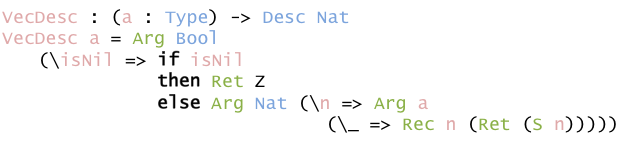
\includegraphics[scale=0.5]{Figures/VectorDescription.png}
\end{center}
\caption{Described version of Vec}
\label{fig:descvec}
\end{figure}

The astute reader might have some questions at this point such as: how is it possible to choose between different constructors? where do parameters go in the description? and why is there only one type for indicies?
I will now try to answer these questions using Figure~\ref{fig:descvec}.

Since we are working in a dependently-typed language, it is possible to encode the choice between constructors by taking one or more multiple arguments and then return the desired description depending on what value is received.
For example, in Figure~\ref{fig:descvec} we take a boolean argument \texttt{isNil} deciding whether the resulting data should be a \texttt{Nil} or \texttt{Cons} and thereafter returning the fitting description.
As this is a fairly primitive encoding, I will present a better but more complex encoding in Section~\ref{sec:TheGenericStructureofInductiveDataTypes} which permits choosing a constructor using its tag.

Regarding parameters, they might not necessarily be required to be encoded in the description datatype itself since they do not change value.
Instead, they may merely be given as function arguments when writing the description of a particular datatype such as in the case of Figure~\ref{fig:descvec}.

Finally for the index, only one type is required since we can represent arbitrary number of index arguments using a dependent pair by uncurrying. For example, for a type constructor with signature
\texttt{(n : Nat) -> Fin n -> Type}, i.e. with indices \texttt{Nat} and \texttt{Fin n}, it is possible to just uncurry the indicies such that they are \texttt{(n : Nat ** Fin n)} and so forth for more complicated indicies.

Now that the interesting questions has been answered, let us in the end try and get an overview of Figure~\ref{fig:descvec}. As mentioned, the description starts with a boolean argument \texttt{isNil} that we use to check for which constructor
we want to create, i.e. either \texttt{Nil} or \texttt{Cons}. If we are trying to construct a \texttt{Nil} which doesn't contain any data then we simply use \texttt{Ret} stating that the description is finished with the index of the resulting type being \texttt{Z}, analogously to Figure~\ref{fig:anatomydatatype}.
In the case of \texttt{Cons} we first take a \texttt{Nat} argument to be used for the necessary indices, similarly to Figure~\ref{fig:anatomydatatype} but this time explicitly.\footnote{Implicit arguments is a feature of Idris that only works on top-level declarations}. Afterwards we take an argument of the input parameter type \texttt{a}, and a recursive argument---this time specified using \texttt{Rec} instead of \texttt{Arg}---that must satisfy to have \texttt{n} as index, i.e. the argument must be of type \texttt{Vect a n}.
Finally we finish the description with \texttt{Ret} and specify that the resulting index must be \texttt{S n} as expected.

\section{Problem Definition}
\label{sec:ProblemDefinition}

The current work on generic programming in dependently-typed languages presents both elegant and correct ways to represent the structural descriptions of datatypes.
Yet in many areas the work that has been done is mostly theoretically oriented, which can lead to some issues when used in a practical manner.
First of all, many authors often use multiple incompatible descriptions depending on what property they would like to show; however this is not particularly attractive in a practical setting, since this could potentially confuse the generic programmer and make it harder for the compiler
to handle transformations from generic programs to ordinary programs, and vica versa.
Secondly, there has been little work on how to integrate such descriptions in more practical languages such as Idris which contains many modern language features such as Type Classes where some operations might be hand-written on some substructures and may not exist at the time of defining a particular generic function.
Finally, datatypes synthesised from descriptions create large canonical terms and as such both type checking and runtime performance is very slow.

\section{Aim and Scope}
\label{sec:AimandScope}
The main aim of this research is to provide a practical and efficient implementation of described types in Idris.

One key part is therefore to find a good definition of the description datatype that supports many of the commonly used datatypes in Idris.
I seek to mainly base my effort on reusing some of the existing work on descriptions, and not try to extend support for other inductive families such as inductive-inductive and inductive-recursive datastypes; neither will I focus on supporting all of the vast language features of Idris such as implicit arguments or codata definitions.
Another key part is to present realistic examples using generic functions by implementing a mechanism for type class deriving and a Scrap Your Boilerplate library for generic querying and traversal.
In the end, I seek to use partial evaluation to optimise the generic functions with regards to specific descriptions to achieve near hand-written performance metrics.

\section{Significance}
\label{sec:Significance}
\begin{itemize}
  \item To show the applicability of generic programming using described types to real-world programs
  \item To show that generic programming using described types can be a viable option to reduce boiler-plate without significant cost in performance
  \item To highlight possible problems in the type-class deriving and generic traversal/querying examples which can be considered future work
\end{itemize}
\section{Overview}
\label{sec:Overview}
\begin{itemize} %Note: Change to non-passive/active I/We voice.
  \item Chapter~\ref{cha:GenericProgramming} highlights the recent developments in generic programming, specifically focusing on described types in dependently-typed programming languages.
  \item Chapter~\ref{cha:PartialEvaluation} investigates techniques for partial evaluation of functions and specialisation of data-type constructors.
  \item Chapter~\ref{cha:LevitatingIdris} discusses further on how the general ideas of levitation, are implemented specifically in an Idris context. Furthermore it discusses, how some of the existing structures,
    can be changed to have descriptions.
  \item Chapter~\ref{cha:OptimizingIdrisforFlight} continues the discussion from Chapter~\ref{cha:LevitatingIdris}, this time concentrating on how optimizations are made
    to ensure that described types do not carry a large run-time overhead.
  \item Chapter~\ref{cha:PracticalExamples} shows two realistic examples for using levitation in Idris, namely type-class deriving and generic traversal/querying.
  \item Chapter~\ref{cha:Evaluation} compares the performance of hand-written data types and functions, with the performance of generic programs on described types.
  \item Chapter~\ref{cha:Discussion} discusses what challenges still lie ahead for practical usage of generic programming using described types, and concludes on the results of this work.
\end{itemize}
\chapter{Generic Programming}
\label{cha:GenericProgramming}
\section{The Generic Structure of Inductive Data Types}
\label{sec:TheGenericStructureofInductiveDataTypes}
\textit{How Generic Programming generally works.}
\section{The Importance of Genericity in Dependently-typed Languages}
\label{sec:TheImportanceofGenericityinDependently-typedLanguages}
\textit{The similarity of structure and various slightly-different indexing of types.}
\section{The (Mostly) Gentle Art of Levitation}
\label{sec:TheMostlyGentleArtofLevitation}
\textit{The elegance of a complete theorem for both ordinary and generic programming. Highlighting of possible issues with performance.}
\chapter{Partial Evaluation}
\label{cha:PartialEvaluation}
\section{Functions and Constant Inputs}
\label{sec:FunctionsandConstantInputs}
\textit{General introduction about partial evaluation.}
\section{Binding-time Analyses of Programs}
\label{sec:Binding-timeAnalysisofPrograms}
\textit{Finding the relevant constant parts of the program.}
\section{Specialisation as a Form of Optimization}
\label{sec:SpecialisationasaFormofOptimization}
\textit{Performance benefits of program specialisation. Pitfalls.}
\chapter{Levitating Idris}
\label{cha:LevitatingIdris}
\section{A Pragmatic Implementation of Levitation}
\label{sec:APragmaticImplementationofLevitation}
\textit{How the general concept of levitation was transferred to Idris.}
\section{Description Synthesis from Ordinary Data Declarations}
\label{sec:DescriptionSynthesisFromOrdinaryDataDeclarations}
\textit{How ordinary data-declarations are synthesized to levitational descriptions.}
\chapter{Optimizing Idris for Flight}
\label{cha:OptimizingIdrisforFlight}
\section{Specialising Constructors for Specific Types}
\label{sec:SpecialisingConstructorsforSpecificTypes}
\textit{How generalized constructors of described types, are specialised as ordinary data structures.}
\section{Online Erasure of Unused Arguments}
\textit{How some type infromation is to be erased at compile time to reduce elaboration overhead. Very hypothetical.}
\label{sec:OnlineErasureofUnusedArguments}
\section{Static Initialization of Generic Functions}
\label{sec:StaticInitializationofGenericFunctions}
\textit{How algorithms that are dependent on the generic structure of a data-type are optimized. Discuss benefits of having a JIT/Profiling information for future work.}
\chapter{Practical Examples}
\label{cha:PracticalExamples}
\section{Generic Deriving}
\label{sec:GenericDeriving}
\textit{Examples of generic deriving of algorithms like decidable equality, pretty printing and possibly eliminators via generic structure.}
\section{Uniplate for Idris}
\label{sec:UniplateforIdris}
\textit{A version of the Uniplate library for Idris based on} \url{http://community.haskell.org/~ndm/uniplate/} \textit{and} \url{http://www-ps.informatik.uni-kiel.de/~sebf/projects/traversal.html} \textit{.
This is useful for traversing structures in a generic fashion and especially when dealing with small changes in large data structures (such as compiler ADTs)}
\chapter{Evaluation}
\label{cha:Evaluation}
\chapter{Discussion}
\label{cha:Discussion}
\section{Future Work}
\label{sec:FutureWork}
\section{Conclusion}
\label{sec:Conclusion}

\end{document}
